\chapter{ERP Analysis}
%\addcontentsline{toc}{chapter}{ERP Analysis}	

Our first analysis of the data followed a strategy similar to the one used in Schaefer \etal \citeyear{schaefer_name_2011}.
Schaefer \etal \citeyear{schaefer_name_2011} used short stimuli (3.26s) allowing each stimulus to be repeated many times and the data to be averaged across hundreds of short trials. 
The grand average \acp{ERP} were concatenated and subjected to a \ac{PCA}, yielding clearly defined spatial features. 
The differences in the time courses of these components were used to classify their stimuli. 
We tried to replicate these results, using the time courses of components derived from the average of the first 3.26 seconds of each of our stimuli. 
We were unable to achieve significant classification results, likely because of our small number of stimuli repetitions.
Therefore, to preserve as much data as possible we conducted a second \ac{PCA} using the full length of the trials as opposed to the first 3.26 seconds. 
We computed grand average \acp{ERP} for each stimulus by averaging the full length trials (excluding the cue).
We then concatenated the grand average \acp{ERP} and applied a \ac{PCA}. 
This resulted in principle components with poorly defined spatial components in \autoref{fig:components} (A and B).
\begin{figure}[htb]	%[htbp] is the default: here, top of page, bottom of page, page by itself
  \centerline{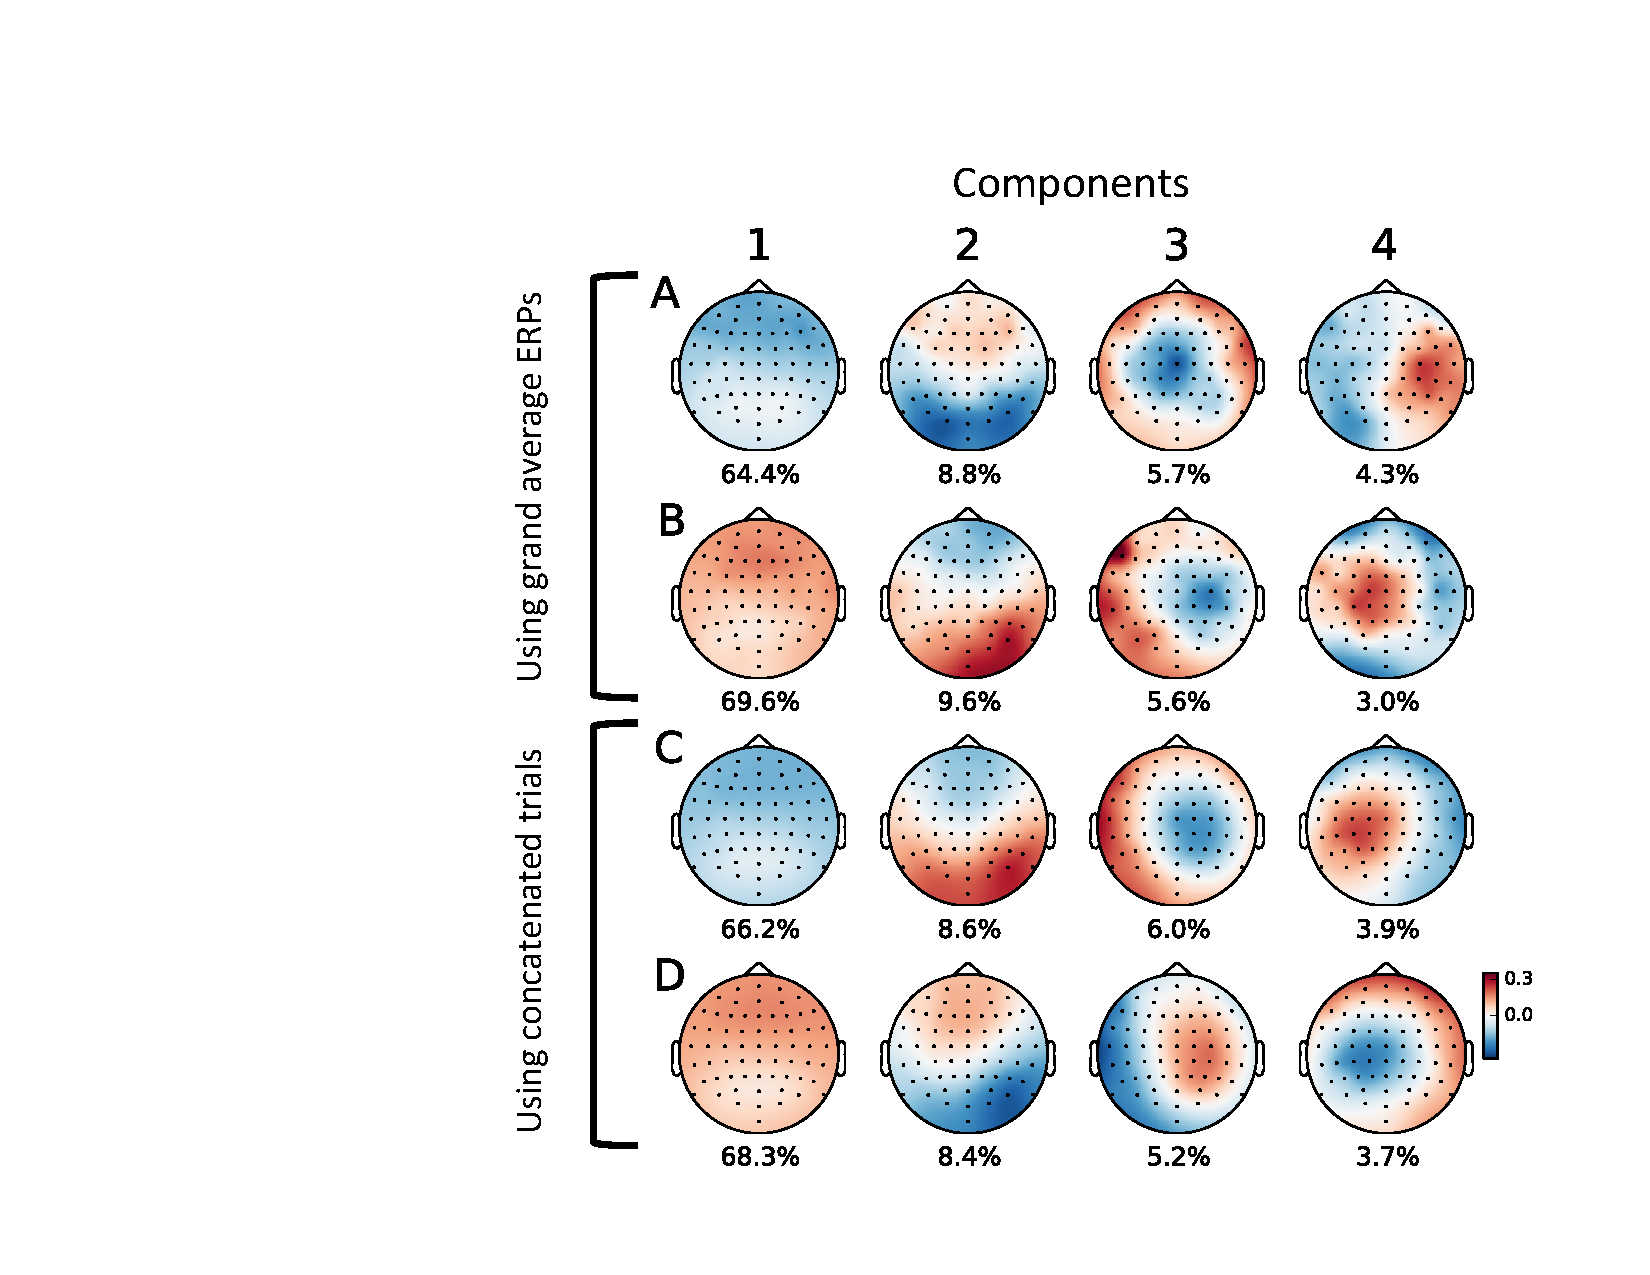
\includegraphics[width=0.7\textwidth]{Figures/principal_components_labels.pdf}}
  \caption{Topographic visualization of the top 4 principle components with percentage of the explained signal variance. Channel positions in the 64-channel EEG layout are shown as dots. Colors are interpolated based on the channel weights. The PCA was computed on {\bf A}: the grand average \acp{ERP} of all perception trials; {\bf B}: the grand average \acp{ERP} of all cued imagination trials; {\bf C}: the concatenated perception trials; {\bf D}: the concatenated cued imagination trials.}
  \label{fig:components}
\end{figure}

In this experiment, we have a small amount of data, and when we calculated grand average \acp{ERP} some of the data was lost which could have negatively impacted the \ac{PCA} results.
To preserve as much of the data as possible, we took an alternative approach. 
All of the raw trials, rather than the averages, were concatenated to create a single, long trial that contained all of the raw EEG information.
We ran a \ac{PCA} on the concatenated raw trials. 
This produced clearly defined spatial components \autoref{fig:components} (C and D).
Except for their (arbitrary) polarity, the components are very similar across perception and imagination, which replicates the results found in \cite{schaefer_name_2011}.

To investigate how similar these components were across conditions and stimuli, we correlated the time courses of component three during perception and imagination.
We used component three as it accounts for the most variance while being similar to a typical auditory component.
The correlation was performed over the first three seconds because we expected the correlations to be highest near the beginning of the trial, before participants's imagination had a chance to drift too far from the cued tempo.
The highest correlations produced by this component were r = 0.40 (p$<$0.001) for ``Eine Kleine Nachtmusic'' (\autoref{fig:nachtmusic})
\begin{figure}[htbp]
  \centerline{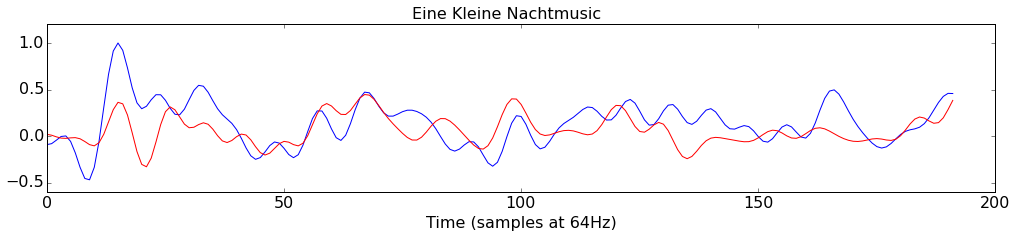
\includegraphics[scale=0.4]{Figures/EineKleineCorrelation}}
  \caption{The time course of component three during perception (blue) and imagination (red) of Eine Kleine Nachtmusic. The correlation between the two time courses is r = 0.40 (p$<$0.001).}
  \label{fig:nachtmusic}
\end{figure}
and r = 0.30 (p$<$0.001) for ``The Emperor Waltz'' (\autoref{fig:emperor}).
\begin{figure}[htbp]
  \centerline{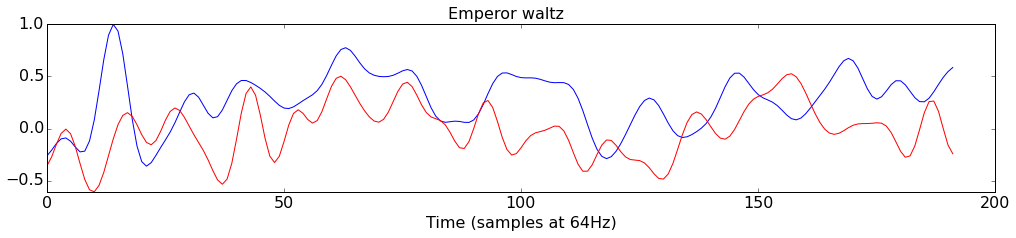
\includegraphics[scale=0.4]{Figures/EmperorCorrelation}}
  \caption{The time course of component three during perception (blue) and imagination (red) of The Emperor Waltz. The correlation between the two time courses is r = 0.30 (p$<$0.001).}
  \label{fig:emperor}
\end{figure}
Although these correlations seem promising for stimulus classification, the perception of Eine Kleine Nachtmusic also correlated well with the imagination of Jingle Bells without lyrics (r = 0.30). 
The highest correlation of r = 0.52 (p$<$0.001) occurred between the imagination of Jingle Bells (without lyrics) and the perception of the Star Wars theme \autoref{fig:starjingle}.
\begin{figure}[htbp]
  \centerline{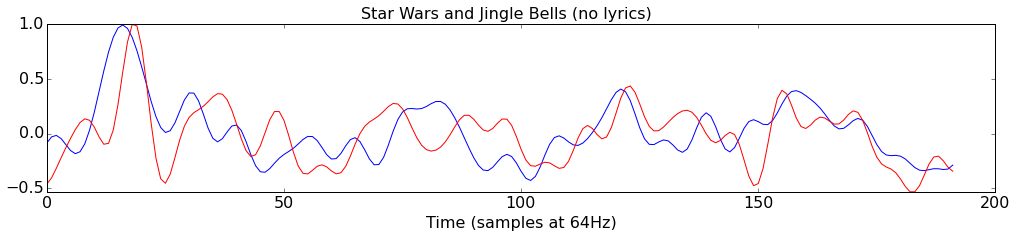
\includegraphics[scale=0.4]{Figures/StarJingle}}
  \caption{The time course of component three during perception (blue) of the Star Wars theme and imagination (red) of Jingle Bells (no lyrics). The correlation between the two time courses is r=0.52 (p$<$0.001).}
  \label{fig:starjingle}
\end{figure}
Because high correlations occurred between trials from different stimuli we could not use this approach to classify our stimuli.
%\hl{include a Table of correlations? with Component 2? component 3?}

Our inability to accurately classify stimuli using this technique could be caused by our much smaller number of trials.
We only had 5 trials per stimulus, ranging from 6.9s to 16s, while Schaefer et al. (2011) collected 145 trials of each of their stimuli, each approximately 3s long.